%Autor: Samuel Kudla <xkudlas00@stud.fit.vutbr.cz>
% Tento súbor je upravená šablóna dostupná na: https://www.fit.vut.cz/study/theses/bachelor-theses/.cs
\chapter{Prehľad sieťových spojení aplikácií}

V nasledujúcej tabuľke je uvedený počet spojení pre jednotlivé aplikácie (celkovo 43 aplikácií) s celkovým počtom 15\,074 spojení. Každá aplikácia má uvedený počet spojení v dátovej sade a pre každý zakódovaný parameter počet unikátnych hodnôt (stĺpce SNI, SrcPort, Ciph, Ext., Gr.).

\begin{longtable}{lrrrrrr}
\caption{Detailný prehľad dostupupnej dátovej sady} \label{tab:app_connections} \\
\toprule
\textbf{Aplikácia} & \textbf{Spojenia} & \textbf{SNI} & \textbf{SrcPort} & \textbf{Ciph.} & \textbf{Ext.} & \textbf{Gr.} \\ \midrule
\endfirsthead

\multicolumn{7}{c}%
{{\bfseries \tablename\ \thetable{} -- pokračovanie z predchádzajúcej strany}} \\
\toprule
\textbf{Aplikácia} & \textbf{Spojenia} & \textbf{SNI} & \textbf{SrcPort} & \textbf{Ciph.} & \textbf{Ext.} & \textbf{Gr.} \\ \midrule
\endhead

\midrule
\multicolumn{7}{r}{{Pokračuje na ďalšej strane}} \\
\bottomrule
\endfoot

\bottomrule
\endlastfoot

AirDroidAirDroid         & 1774 & 43 & 149 & 2 & 3 & 17 \\
OerOer                 & 1441 & 24 & 185 & 3 & 5 & 17 \\
BiduTerBox             & 1252 & 21 & 168 & 3 & 4 & 18 \\
AdmntMessenger         & 1180 & 23 & 115 & 1 & 3 & 16 \\
OenMedi4KStogrm        & 1020 & 27 & 109 & 1 & 2 & 16 \\
OenMedi4KTokkit        & 1012 & 27 & 113 & 1 & 2 & 16 \\
TemSonrrSonrr          & 717  & 14 & 92  & 2 & 3 & 17 \\
MozillFirefox          & 637  & 19 & 110 & 3 & 4 & 3  \\
EstmobSendAnywhere     & 607  & 54 & 120 & 4 & 5 & 17 \\
HedsetHedset           & 554  & 17 & 546 & 3 & 5 & 17 \\
EvernoteEvernote       & 469  & 13 & 47  & 2 & 3 & 17 \\
TIDALMusiASTIDAL       & 365  & 9  & 64  & 1 & 2 & 16 \\
BeeerBeeer             & 342  & 10 & 76  & 1 & 2 & 16 \\
RkutenViber            & 300  & 9  & 100 & 2 & 3 & 1  \\
GoogleChrome           & 287  & 8  & 58  & 2 & 3 & 17 \\
NotionNotion           & 263  & 7  & 71  & 2 & 3 & 33 \\
DeezerDeezer           & 262  & 7  & 77  & 2 & 2 & 17 \\
MozillThunderbird      & 253  & 9  & 56  & 2 & 3 & 2  \\
AsnAsn                 & 248  & 4  & 53  & 2 & 4 & 32 \\
CrineCrine             & 232  & 7  & 64  & 2 & 3 & 17 \\
SlkTehnologiesSlk      & 214  & 5  & 58  & 2 & 2 & 17 \\
SotifySotify           & 199  & 6  & 61  & 1 & 1 & 16 \\
BrveBrve               & 150  & 5  & 34  & 1 & 2 & 16 \\
NotionNotionClendr     & 145  & 6  & 43  & 1 & 1 & 16 \\
BiglySoftwreBiglyBT    & 141  & 6  & 50  & 2 & 2 & 2  \\
LINELINE               & 95   & 4  & 33  & 2 & 4 & 2  \\
TymnixEletorrent       & 79   & 4  & 78  & 3 & 3 & 16 \\
CloudAGCloudDrive      & 78   & 5  & 42  & 2 & 3 & 1  \\
OenWhiserSystemsSignl  & 77   & 2  & 21  & 1 & 1 & 1  \\
ZoomZoom               & 75   & 1  & 21  & 1 & 1 & 1  \\
MirosoftEdge           & 75   & 6  & 43  & 1 & 1 & 1  \\
CozyCloudCozyDrive     & 72   & 2  & 31  & 1 & 1 & 15 \\
eMClienteMClient       & 72   & 2  & 17  & 1 & 1 & 1  \\
TrillinTrillin         & 72   & 2  & 20  & 1 & 1 & 1  \\
ProtonProtonDrive      & 72   & 2  & 35  & 1 & 1 & 1  \\
YndexMessenger         & 72   & 2  & 31  & 1 & 1 & 1  \\
NextloudNextloudDeskto & 36   & 1  & 15  & 1 & 1 & 1  \\
MehediHssnTweeten      & 36   & 1  & 26  & 1 & 1 & 14 \\
MegMEGASyn             & 35   & 0  & 25  & 1 & 1 & 1  \\
SlshedIoInssist        & 27   & 2  & 21  & 2 & 2 & 15 \\
TemDriveSystemsTemDrive& 21   & 1  & 10  & 1 & 1 & 1  \\
MilbirdMilbird         & 15   & 2  & 8   & 2 & 2 & 1  \\
TelegrmTelegrmDeskto   & 1    & 1  & 1   & 1 & 1 & 1  \\ \midrule
\textbf{Celkom}        & \textbf{15 074} & \multicolumn{5}{l}{} \\
\end{longtable}

\begin{figure}[h]
    \centering
    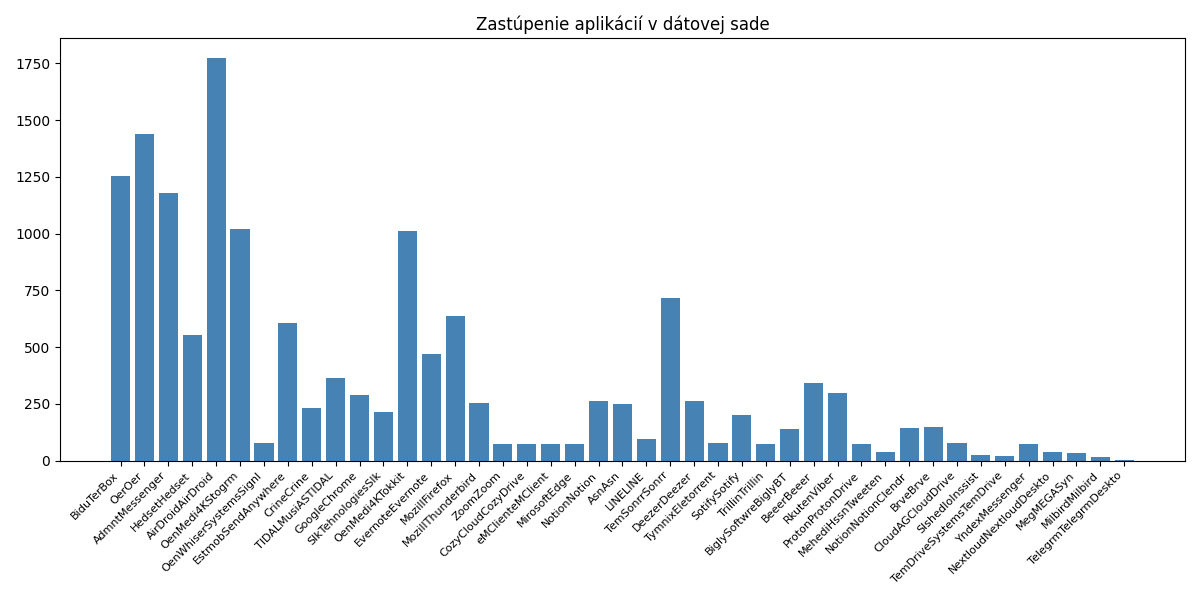
\includegraphics[width=1\linewidth]{obrazky-figures/all_apps_count_full.png}
    \caption{Grafické zobrazenie zastúpení jednotlivých aplikácií v dostupnej dátovej sade}
    \label{graph:all_apps_count}
\end{figure}
\newpage

%%%%%%%%%%%%%%%%%%%%%%%%%%%%%%%%%%%%%%%%%%%%%%%%%%%%%%%%%%%%%%%%%
%%%%%%%%%%%%%%%%%%%%%%%%%%%%%%%%%%%%%%%%%%%%%%%%%%%%%%%%%%%%%%%%%
%%%%%%%%%%%%%%%%%%%%%%%%%%%%%%%%%%%%%%%%%%%%%%%%%%%%%%%%%%%%%%%%%%%%%%%%%%%%%%%%%%%%%%%%%%%%%%%%%%%%%%%%%%%%%%%%%%%%%%%%%%%%%%%%%%

\begin{longtable}{lc}
\caption{Štatistický prehľad unikátnych hodnôt v datasete} \label{tab:unique_entries} \\
\toprule
\textbf{Parameter} & \textbf{Unikátne záznamy} \\ \midrule
\endfirsthead

\multicolumn{2}{c}%
{{\bfseries \tablename\ \thetable{} -- pokračovanie z predchádzajúcej strany}} \\
\toprule
\textbf{Parameter} & \textbf{Unikátne záznamy} \\ \midrule
\endhead

\midrule
\multicolumn{2}{r}{{Pokračuje na ďalšej strane...}} \\
\bottomrule
\endfoot

\bottomrule
\endlastfoot

SrcIP & 1252 \\
DstIP & 892 \\
SrcPort & 822 \\
DstPort & 2 \\
Proto & 1 \\
SNI & 306 \\
OrgName & 109 \\
TLS Version & 1 \\
Client CipherSuite & 14 \\
Client Extensions & 29 \\
Client Supported Groups & 39 \\
EC\_fmt & 2 \\
ALPN & 3 \\
Signature Algorithms & 10 \\
Client Supported Versions & 35 \\
JA3hash & 9415 \\
JA4 hash & 39 \\
JA4\_raw & 39 \\
Type & 3 \\
Server CipherSuite & 9 \\
Server Extensions & 42 \\
Server Supported Versions & 2 \\
JA3S hash & 58 \\
JA4S hash & 60 \\
JA4S\_raw & 60 \\
Version & 2 \\
\end{longtable}

\newpage


\chapter{Prehľad parametrov TLS \textit{Client Hello} správy}
V nasledujúcom zozname je uvedená ukážka štruktúry správy pre extrahované a sformátované vstupné dáta v dostupnom datasete.
\begin{lstlisting}[caption={Ukážka extrahovaných parametrov pre aplikáciu AirDroid}, label={lst:tls_airdroid}]
SrcIP: 172.17.151.209
DstIP: 65.9.95.47
SrcPort: 49751
DstPort: 443
Proto: 6
SNI: img-5-cdn.airdroid.com
OrgName: Amazon.com, Inc., AMAZO-CF
TLS Version: 771
Client CipherSuite: 47-53-156-157-4865-4866-4867-49171-49172-49195-49196-49199-49200-52392-52393
Client Extensions: 0-5-10-11-13-16-18-23-27-35-43-45-51-17513-65037-65281
Client Supported Groups: 0x0017,0x0018,0x001d,0x6399,0x9a9a
ALPN: h2,http/1.1
JA3hash: f9bb5c4d99971efe404e4722def23540
JA4 hash: t13d1516h2_8daaf6152771_02713d6af862
\end{lstlisting}

\chapter{Porovnanie funkčnosti referenčného a upravneného kódovania čisel portov}
V nasledujúcej tabuľke porovnávame výstupy referenčného a upraveného algoritmu s normalizáciou pre kódovanie čisel portov, ktorý bol optimalizovaný na zvýšenie váhy vyšších cifier pri súčasnom zachovaní významu nižších poradových čísel portov.
\begin{table}[H]
    \centering
    \caption{Porovnanie výstupov starého a nového algoritmu pre PortEmbedder triedu}
    \label{tab:port_comparison}
    \begin{tabular}{@{}rrr@{}}
        \toprule
        \textbf{Port} & \textbf{Starý algoritmus} & \textbf{Nový algoritmus} \\ \midrule
        420   & 0.1906202723 & 0.0023615173 \\
        10000 & 0.1210287443 & 0.1627282601 \\
        19999 & 0.6248108926 & 0.2052919290 \\
        20000 & 0.2420574887 & 0.3254565203 \\
        49999 & 0.9878971256 & 0.6934767094 \\
        50000 & 0.6051437216 & 0.8136413007 \\
        55245 & 0.8456883510 & 0.8367857548 \\
        60000 & 0.7261724660 & 0.9763695608 \\
        65535 & 1.0000000000 & 1.0000000000 \\ \bottomrule
    \end{tabular}
\end{table}
\enlargethispage{\baselineskip}

\chapter{Schéma implementácie systému}
\begin{figure}[H]
    \centering
    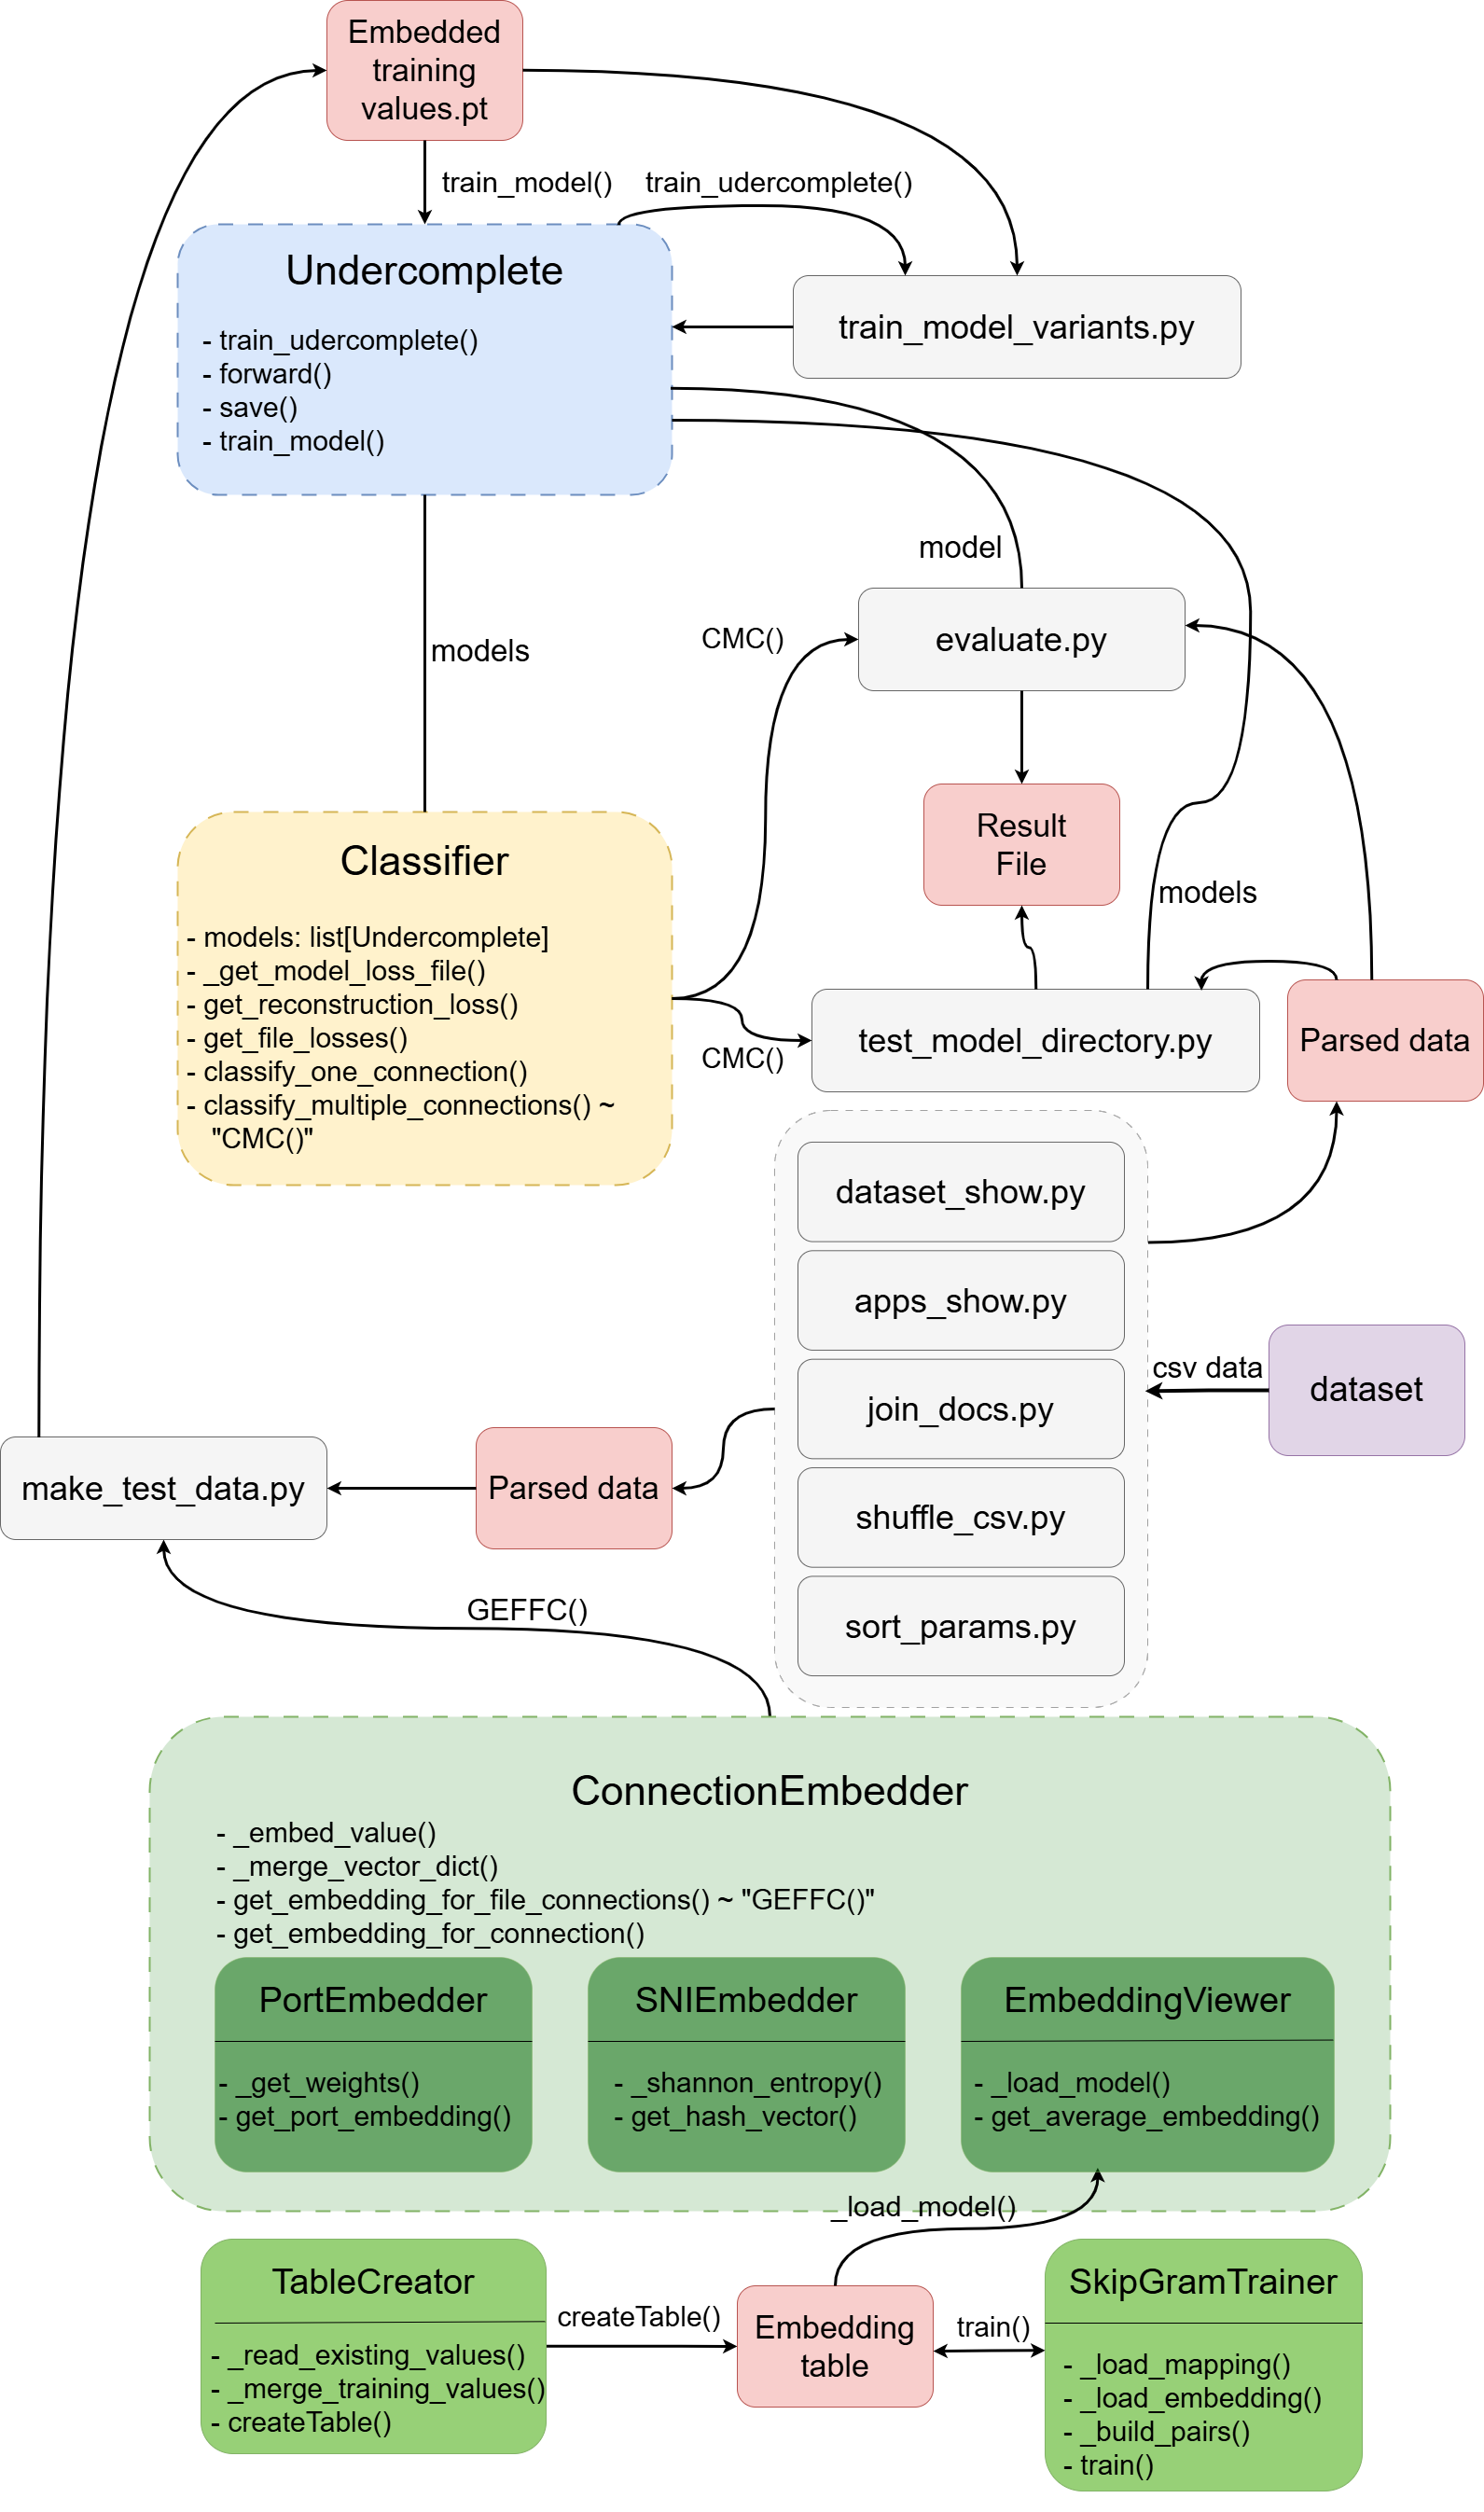
\includegraphics[width=0.59\linewidth]{obrazky-figures/CodeStruct.png}
    \caption{Schéma zobrazujúca skripty a~triedy implementovaného systému.}
    \label{fig:code_struct}
\end{figure}

\chapter{Grafy testovania rôzneho počtu vrstiev modelov}\label{append:layers_structs_graph}
V tejto časti sú graficky zobrazené výsledky testov rôznych štruktúr pre modely aplikácii AirDroid, BiduTerBox, Oer a AdmntMessenger. Na ose x sa celkové nachádzajú počty vrstiev modelu (tzn. skryté vrstvy so vstupnou a výstupnou vrstvou). Úspešnosť modelu je hodnotená MCC koeficientom, pričom sa berie ohľad aj na počet epoch, počas ktorých sa model trénoval, ktorých je definovaný konfiguráciou \textit{early stoppingu} (sekcia~\ref{exp:dynamic_delta})

\begin{figure}[H]
    \centering
    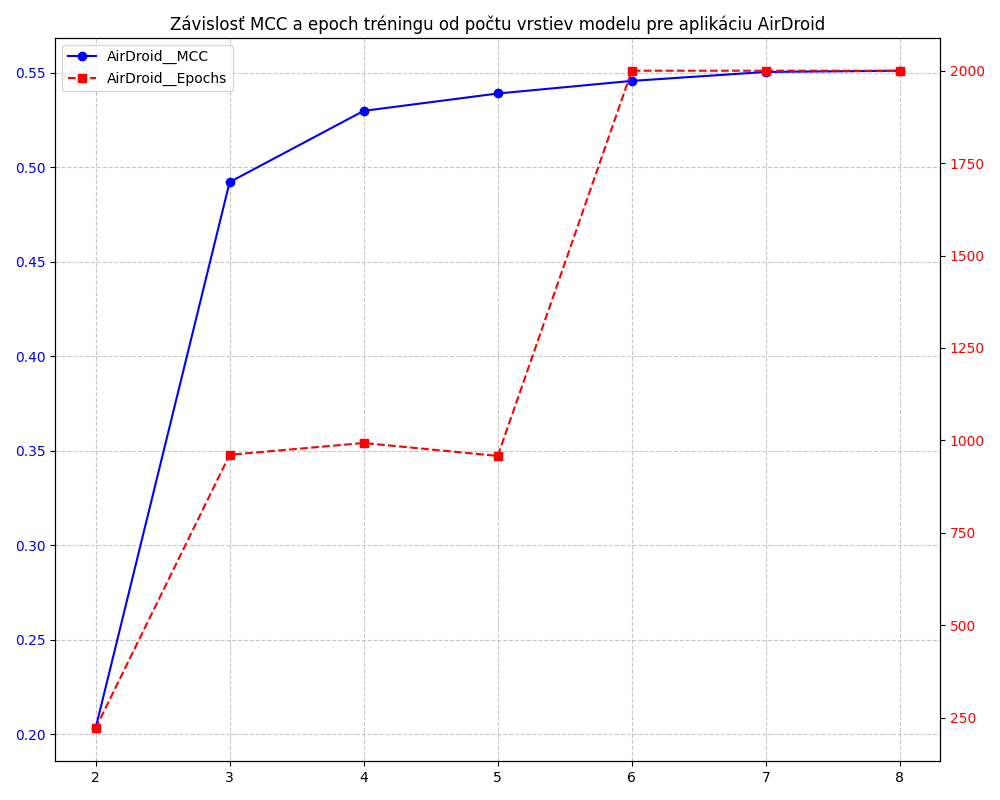
\includegraphics[width=0.75\linewidth]{obrazky-figures/AirDroidMCC.png}
    \caption{Porovnanie vplyvu počtu vrstiev na metriku MCC pre aplikáciu AirDroid.}
    \label{graph:AirDroidLayers}
\end{figure}

\begin{figure}[H]
    \centering
    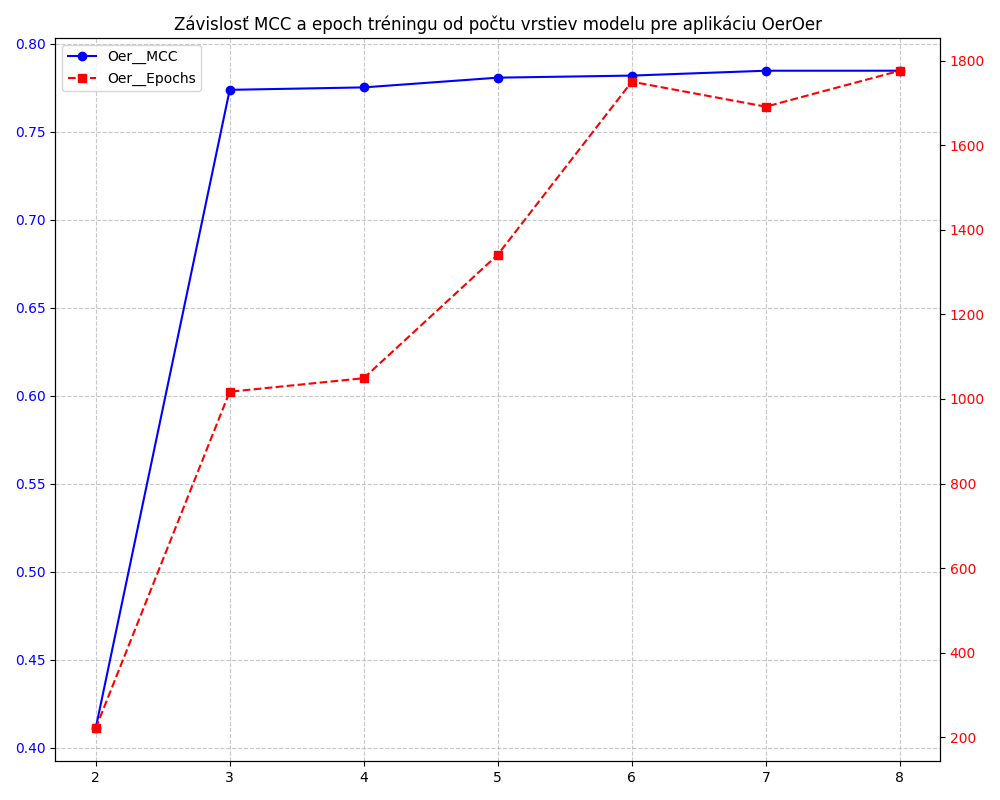
\includegraphics[width=0.75\linewidth]{obrazky-figures/OerMCC.png}
    \caption{Porovnanie vplyvu počtu vrstiev na metriku MCC pre aplikáciu Oer.}
    \label{graph:OerLayers}
\end{figure}

\begin{figure}[H]
    \centering
    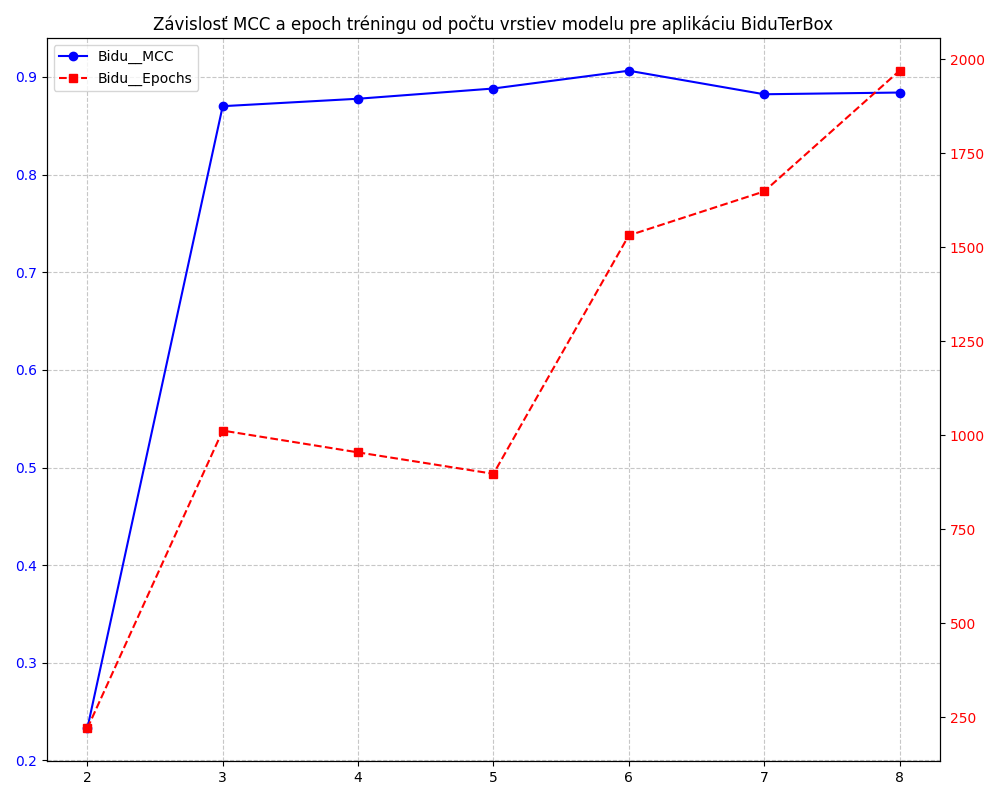
\includegraphics[width=0.75\linewidth]{obrazky-figures/BiduMCC.png}
    \caption{Porovnanie vplyvu počtu vrstiev na metriku MCC pre aplikáciu BiduTerBox.}
    \label{graph:BiduLayers}
\end{figure}

\begin{figure}[H]
    \centering
    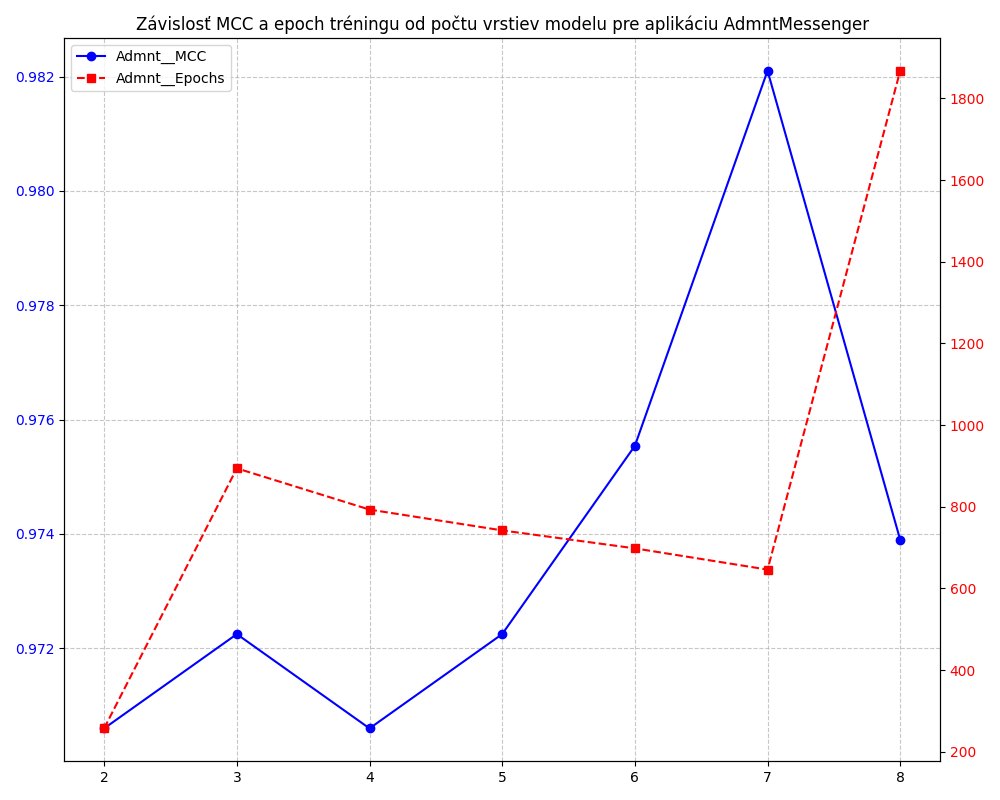
\includegraphics[width=0.75\linewidth]{obrazky-figures/AdmntMCC.png}
    \caption{Porovnanie vplyvu počtu vrstiev na metriku MCC pre aplikáciu AdmntMessenger.}
    \label{graph:AdmntLayers}
\end{figure}

\chapter{Grafy testovania rôznej veľkosti latentného priestoru modelu pre jednu cieľovú aplikáciu}
V tejto časti sú uvedené graficky zobrazené výsledky testov pre modely cieľovej aplikácie AirDroid, pričom každý model obsahuje rôznu dimenziu latentnej vrstvy (zobrazené na osi~x). 

\section{Grafy zobrazujúce závislosť MCC a počtu epoch pre trénovanie modelov od veľkosti latentnej vrstvy}\label{graph:latent_size_graphs}
% --- 4-layers
\begin{figure}[H]
    \centering
    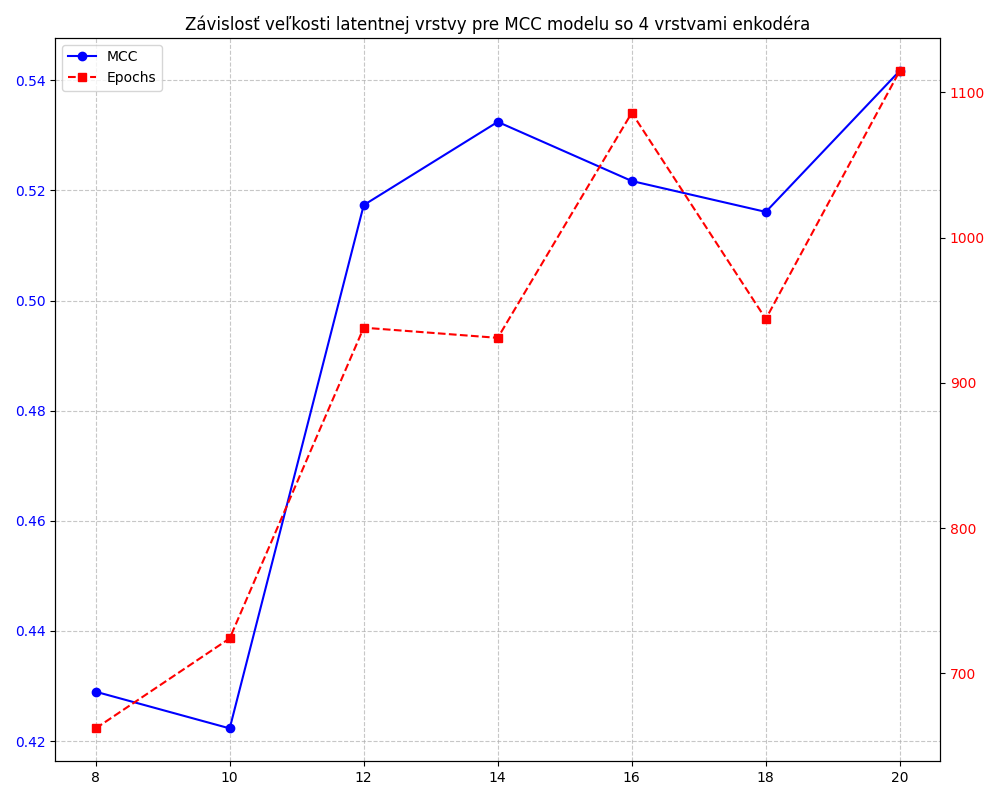
\includegraphics[width=0.75\linewidth]{obrazky-figures/Latent4.png}
    \caption{Vplyv veľkosti bottlenecku na MCC koeficient (4-vrstvový model).}
    \label{graph:Latent4MCC}
\end{figure}

\begin{figure}[H]
    \centering
    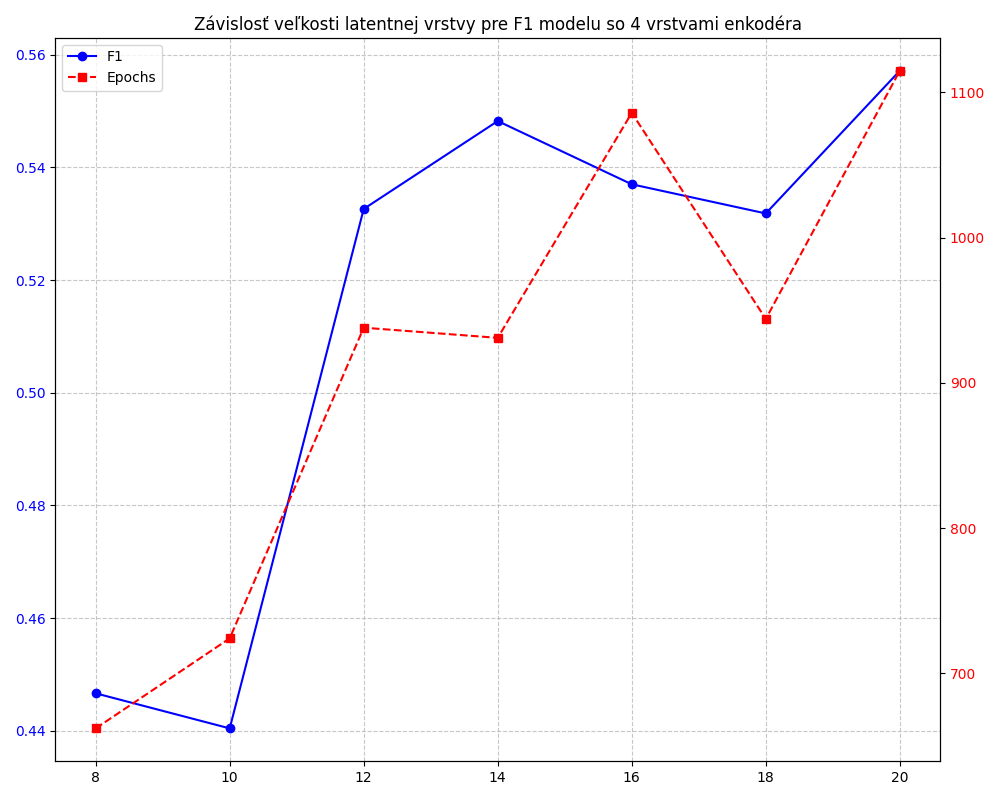
\includegraphics[width=0.75\linewidth]{obrazky-figures/Latent4F1.png}
    \caption{Vplyv veľkosti bottlenecku na F1 skóre (4-vrstvový model).}
    \label{graph:Latent4F1}
\end{figure}

% --- 5-layers
\begin{figure}[H]
    \centering
    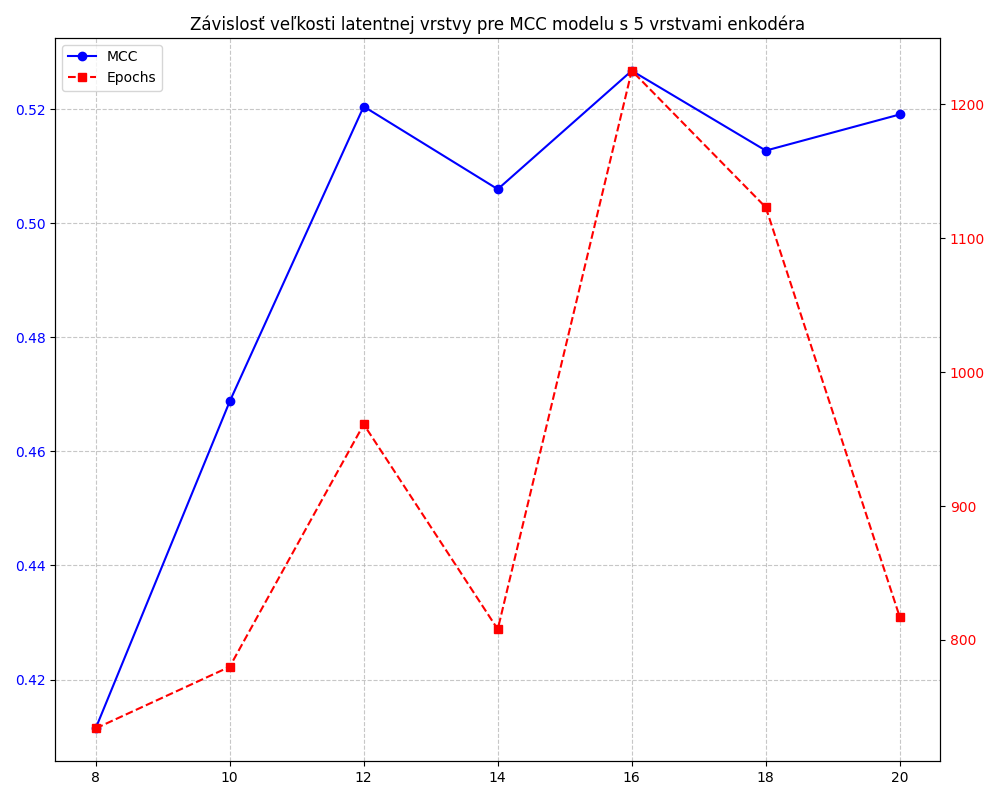
\includegraphics[width=0.75\linewidth]{obrazky-figures/Latent5.png}
    \caption{Vplyv veľkosti bottlenecku na MCC koeficient (5-vrstvový model).}
    \label{graph:Latent5MCC}
\end{figure}

\begin{figure}[H]
    \centering
    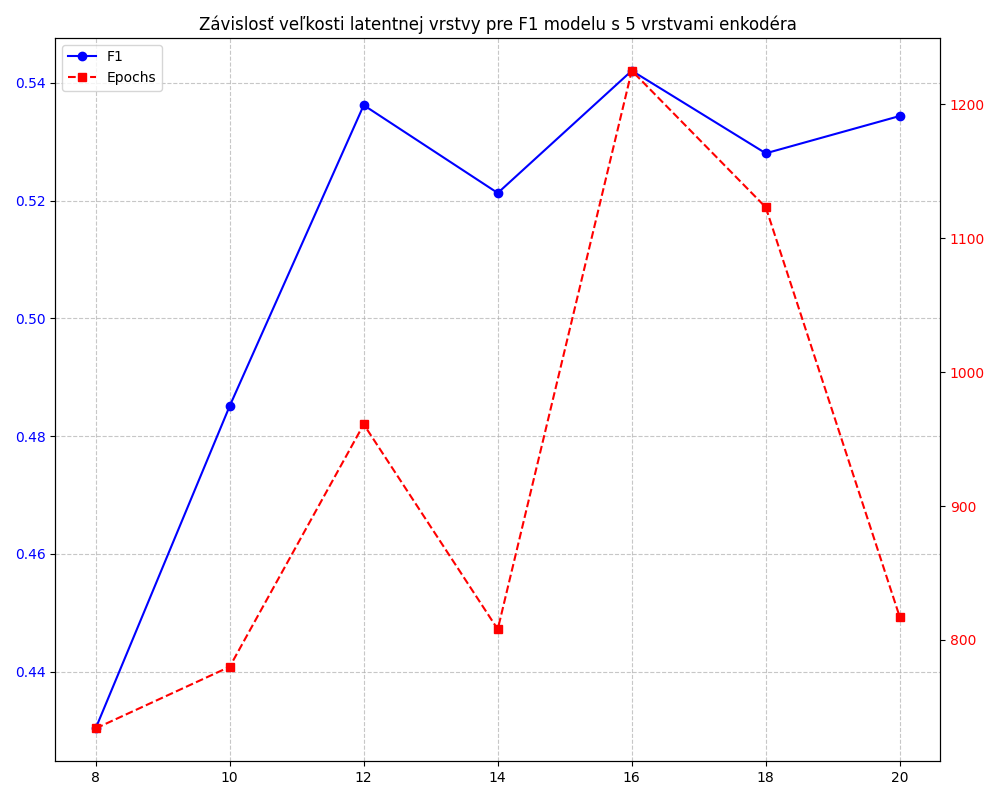
\includegraphics[width=0.75\linewidth]{obrazky-figures/Latent5F1.png}
    \caption{Vplyv veľkosti bottlenecku na F1 skóre (5-vrstvový model).}
    \label{graph:Latent5F1}
\end{figure}

% --- 6-layers
\begin{figure}[H]
    \centering
    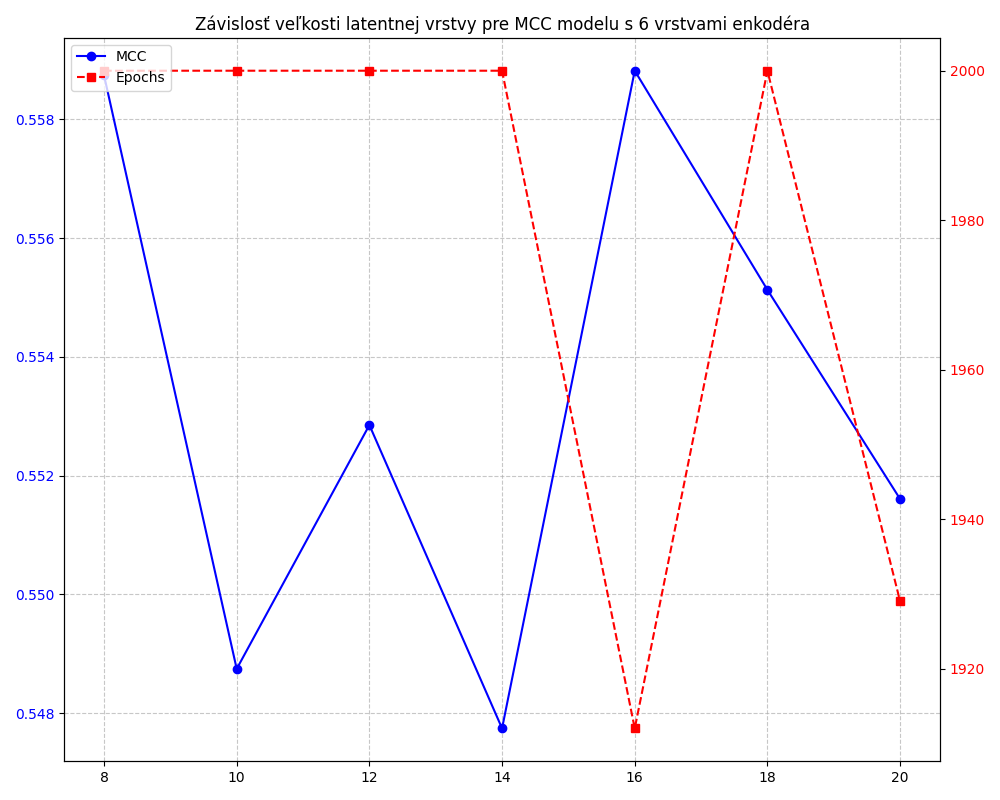
\includegraphics[width=0.75\linewidth]{obrazky-figures/Latent6.png}
    \caption{Vplyv veľkosti bottlenecku na MCC koeficient (6-vrstvový model).}
    \label{graph:Latent6MCC}
\end{figure}

\begin{figure}[H]
    \centering
    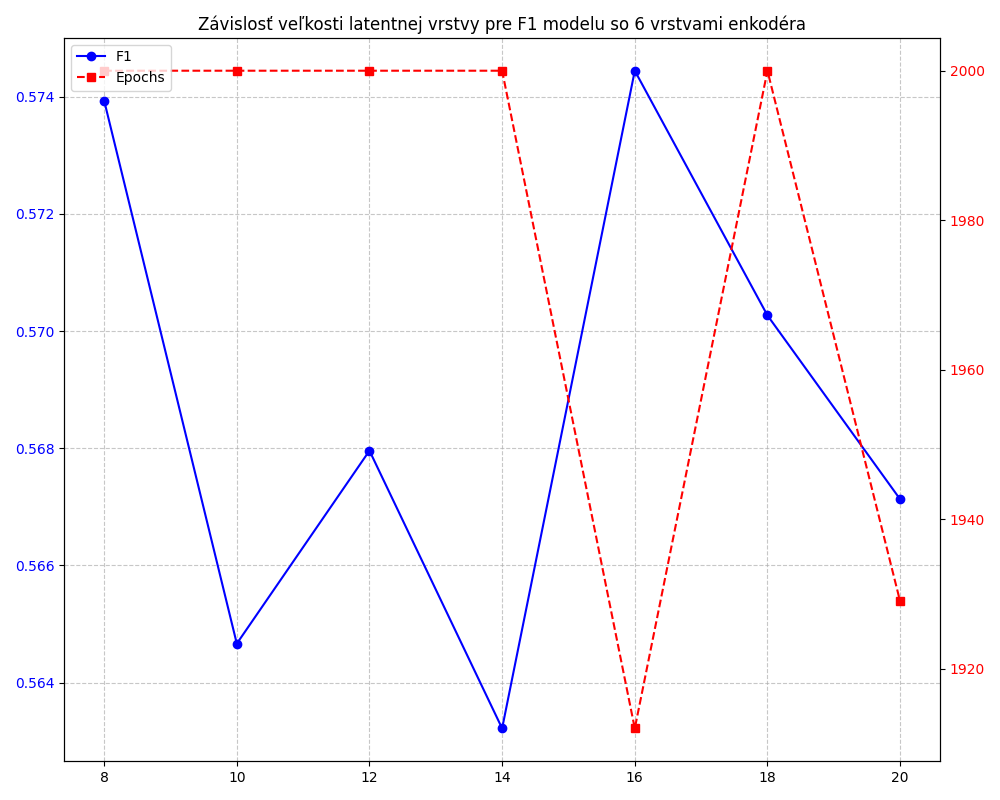
\includegraphics[width=0.75\linewidth]{obrazky-figures/Latent6F1.png}
    \caption{Vplyv veľkosti bottlenecku na F1 skóre (6-vrstvový model).}
    \label{graph:Latent6F1}
\end{figure}


\section{Grafy zobrazujúce závislosť Precision a Recall pre trénovanie modelov od veľkosti latentnej vrstvy}\label{graph:latent_size_graphs_Precision}

\begin{figure}[H]
    \centering
    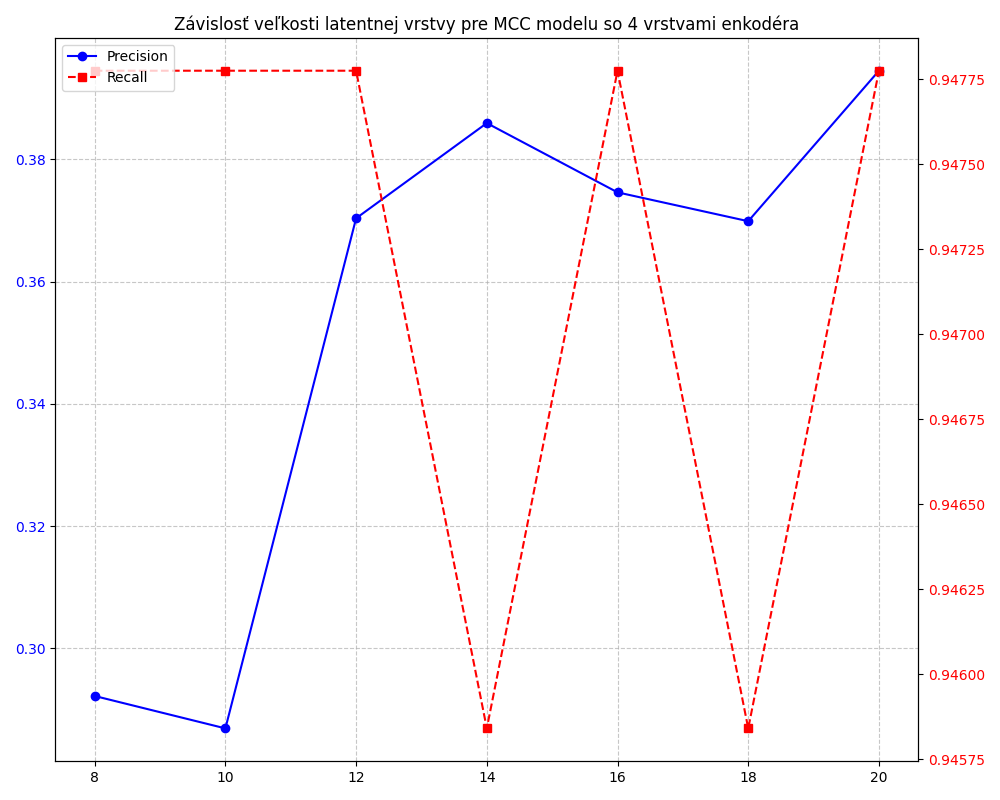
\includegraphics[width=0.75\linewidth]{obrazky-figures/PrecisionRecall4.png}
    \caption{Graf pre model obsahujúci 4 vrstvy v enkodéri.}
    \label{graph:LayersAirDroidPrecision4}
\end{figure}
\begin{figure}[H]
    \centering
    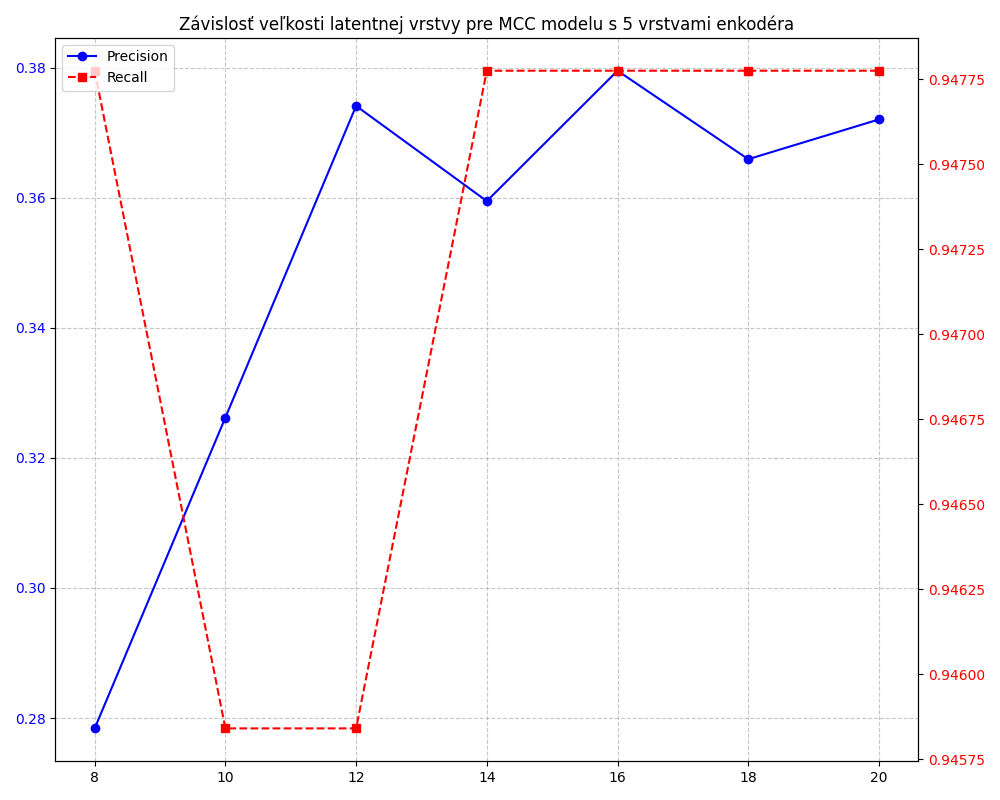
\includegraphics[width=0.75\linewidth]{obrazky-figures/PrecisionRecall5.png}
    \caption{Graf pre model obsahujúci 5 vrstiev v enkodéri.}
    \label{graph:LayersAirDroidPrecision5}
\end{figure}
\begin{figure}[H]
    \centering
    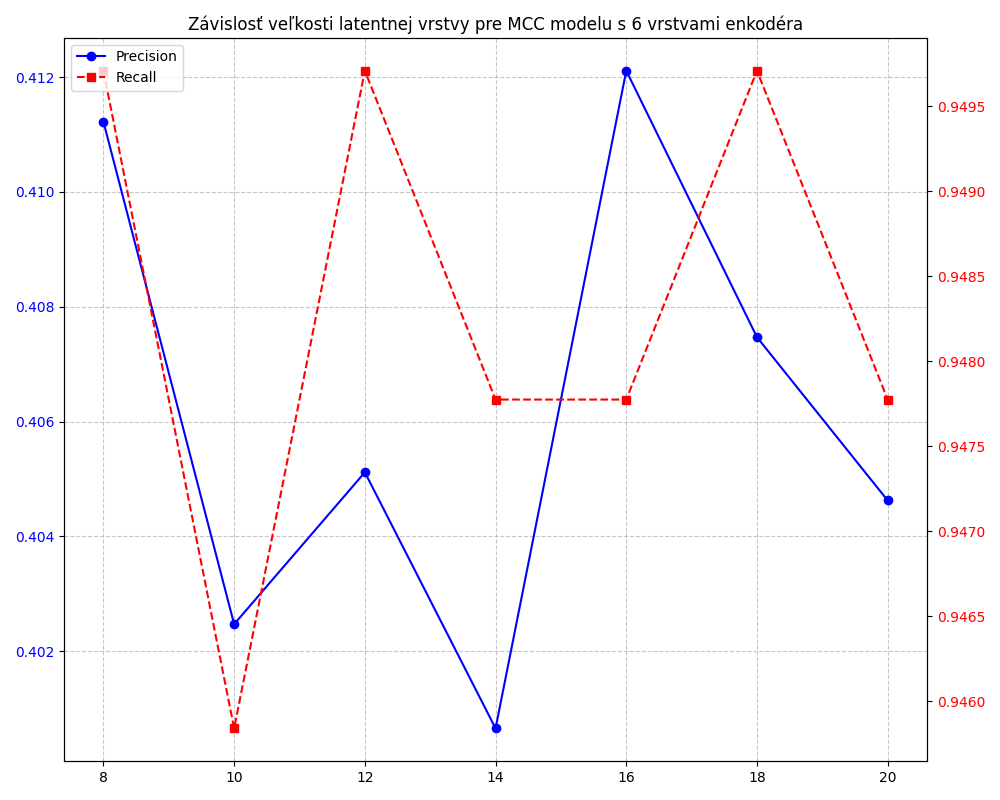
\includegraphics[width=0.75\linewidth]{obrazky-figures/PrecisionRecall6.png}
    \caption{Graf pre model obsahujúci 6 vrstiev v enkodéri.}
    \label{graph:LayersAirDroidPrecision6}
\end{figure}

\chapter{Štatistické výsledky modelov aplikácií}
V tejto časti sú uvedené metriky pre päť vybraných modelov, ktoré boli trénované a testované v rámci systému binárnej klasifikácie pre detekciu konkrétnych aplikácií.

\begin{table}[H]
    \centering
    \caption{Komplexné výsledky binárnej klasifikácie pre jednotlivé modely aplikácií.}
    \label{tab:each_model_all_metrics}
    \small
    \begin{tabular}{lrrrrr}
        \toprule
        \textbf{Metrika} & \textbf{AirDroid} & \textbf{BiduTerBox} & \textbf{OerOer} & \textbf{AdmntMsg} & \textbf{OenMedi4K} \\
        \midrule
        Accuracy [\%]    & 83,96    & 99,06    & 94,63    & 99,30    & 84,89    \\
        Precision        & 0,418    & 0,998    & 0,662    & 1,000    & 0,301    \\
        Recall           & 0,929    & 0,888    & 0,893    & 0,911    & 0,934    \\
        Specificity      & 0,828    & 1,000    & 0,952    & 1,000    & 0,843    \\
        FPR              & 0,172    & 0,000    & 0,048    & 0,000    & 0,157    \\
        F1 Score         & 0,577    & 0,940    & 0,761    & 0,953    & 0,456    \\
        MCC              & 0,555    & 0,937    & 0,741    & 0,951    & 0,479    \\
        \midrule
        Epochy           & 1124     & 1009     & 962      & 1100     & 1158     \\
        Čas tréningu [s] & 15,24    & 14,23    & 11,11    & 13,19    & 12,52    \\
        Chyba testu      & 0,00175  & 0,00109  & 0,00112  & 0,00093  & 0,00111  \\
        Prah             & 0,00296  & 0,00188  & 0,00217  & 0,00165  & 0,00167  \\
        \bottomrule
    \end{tabular}
\end{table}